\subsubsection{Benutzeransicht}
\label{sec:Benutzeransicht}

Ein erster Oberflächenentwurf der Benutzeransicht des vorliegenden Projektes
ist in \abbildung{MockupFrontend} dargestellt.

\begin{figure}[htb]
\centering
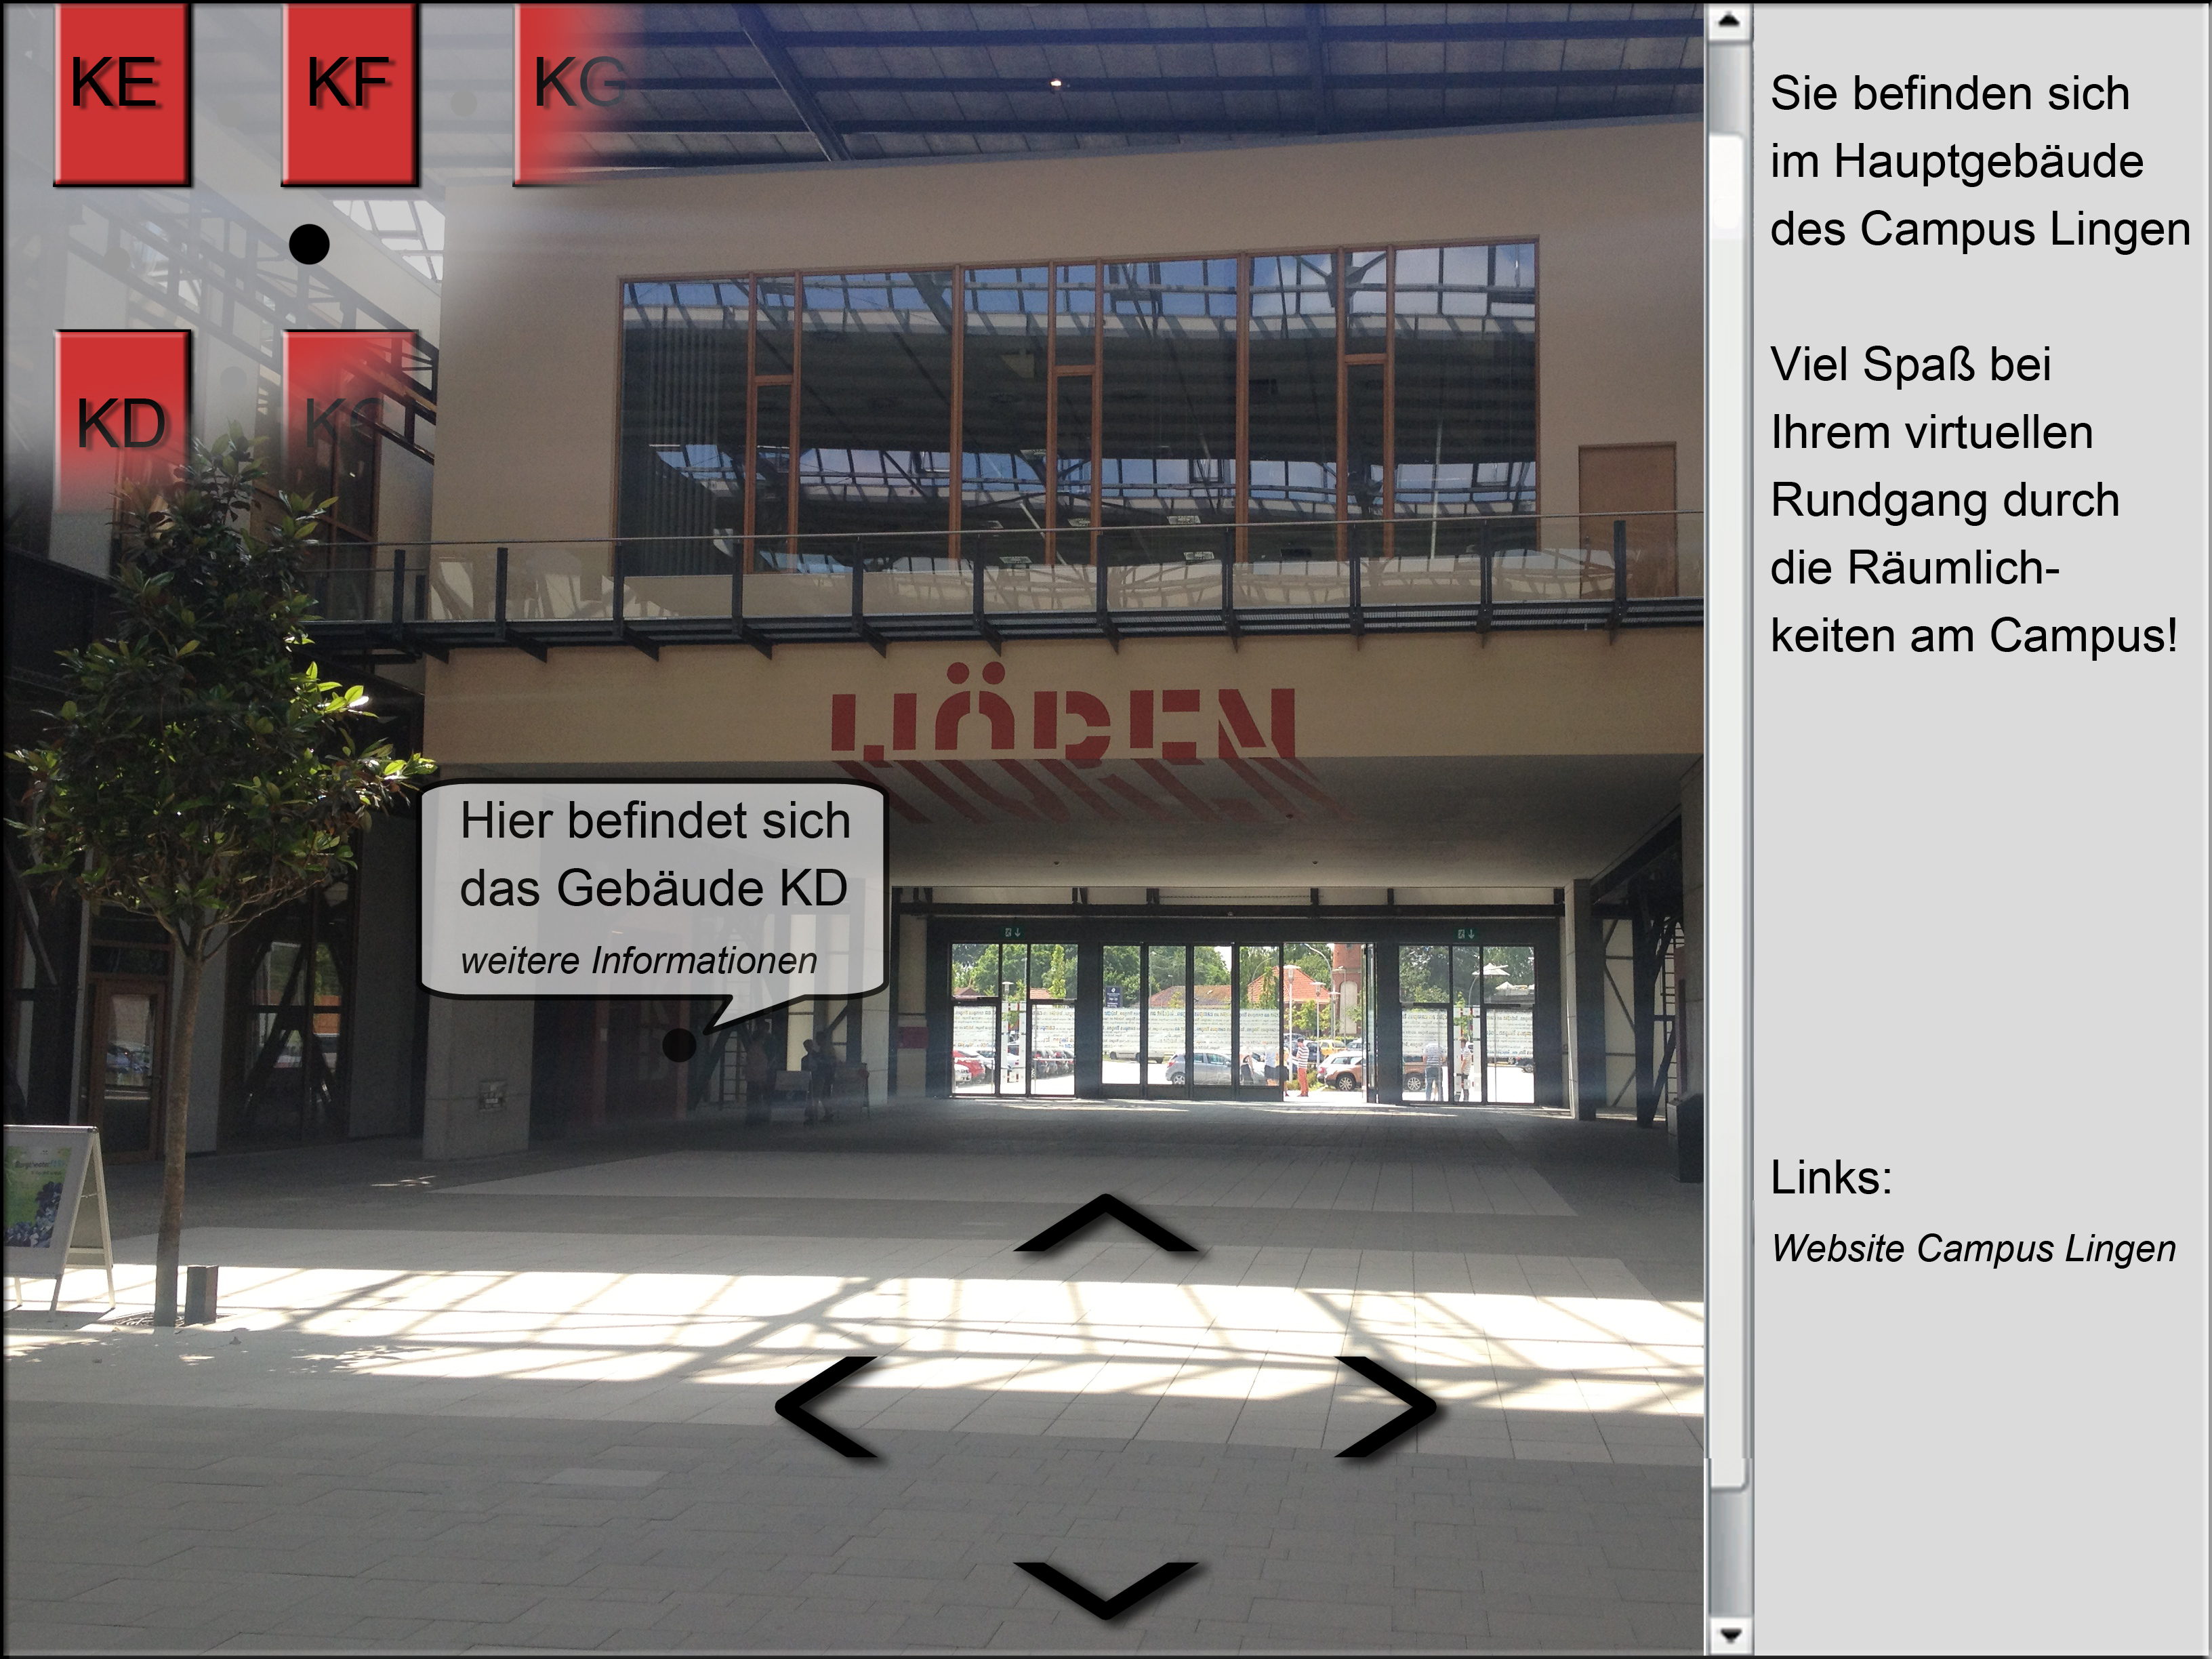
\includegraphics[width=1.0\textwidth]{MockupFrontend.jpg}
\caption[Oberflächenentwurf der
Benutzeransicht]{Oberflächenentwurf der
Benutzeransicht\protect\footnotemark}
\label{fig:MockupFrontend}
\end{figure}
\footnotetext{Quelle: Eigene Darstellung}

\clearpage

In diesem Mockup sind folgende vier Elemente abgebildet:

\begin{itemize}
 \item Ein 360-Grad-Foto
 \item Ein Steuerkreuz
 \item Eine Übersichtskarte (Minimap)
 \item Ein Informationsfenster
\end{itemize}

Das \textbf{360-Grad-Foto} ist hierbei zentrales Element des Projektes. Dieses
Foto stellt einen Standpunkt dar, von dem aus sich der Benutzer den Campus
Lingen ansehen kann. Von diesem Standpunkt aus kann sich der Benutzer in alle
Richtungen in dem Panoramafoto frei umsehen.

Mit dem \textbf{Steuerkreuz} am unteren Rand des dargestellten
Oberflächenentwurfs kann der Benutzer zu einem anderen Aufnahmepunkt wechseln.
Er kann auf diese Weise den Campus von einem anderen Standpunkt aus betrachten.
An diesem neuen Standort kann sich der Benutzer wiederum frei umsehen. Die
Pfeile des Steuerkreuzes zeigen dabei zu jedem Panoramafoto, welches von der
aktuellen Position aus erreichbar ist.

Die \textbf{Minimap} ist in einer Ecke des Panoramas platziert und erfüllt
zwei Aufgaben: Zum einen dient sie der Orientierung des Benutzers. Sie zeigt, an
welcher Aufnahmeposition sich der Benutzer aktuell am Campus
befindet\footnote{Im Oberflächentwurf ist diese Position durch einen schwarzen
Punkt gekennzeichnet.}. Hierdurch wird neben dem Einblick in die Räumlichkeiten
des Campus auch ein Bild vom Aufbau des Campus vermittelt. Zum anderen kann die
Minimap, ähnlich wie die Pfeile des Steuerkreuzes, zum Navigieren zu anderen
Standpunkten genutzt werden. Beim Klicken auf die Minimap öffnet sich ein
Informationsfenster, welches interessante Orte der Hochschule anzeigt. Bei der
Auswahl eines der Orte aus der Liste wechselt die Position des Benutzers zu
dem ausgewählten Standpunkt. Auch der Ausschnitt, der auf der Minimap
präsentiert wird, passt sich der neuen Position des Benutzers an.

Das \textbf{Informationsfenster} zeigt interessante Informationen zum aktuellen
Panorama an. Im obigen Oberflächenentwurf sind zwei solcher Informationsfenster
dargestellt\footnote{Die Informationsfenster befinden sich am rechten Rand
sowie oberhalb des Steuerkreuzes}. Diese Darstellungsformen sind als alternativ
zu betrachten. Die Art der Informationsdarstellung ist zum Zeitpunkt des
Oberflächenentwurfs noch nicht eindeutig festgelegt. Inhalt dieser
Informationsfenster können dabei interessante Projekte einzelner Studiengänge,
Öffnungszeiten von Räumlichkeiten oder Wissenwertes aus dem Studienalltag sein.
Die Informationen sollen in Form eines Popup-Fensters dargestellt werden. Sie
sollen also nicht permanent angezeigt werden, sondern erscheinen erst durch
Klicken des Benutzers auf einen Button. Dadurch wird das Blickfeld des Benutzers
nicht durch störende Anzeigen eingeschränkt.
